\documentclass[12pt, a4paper]{article} % Tamanho da fonte, formato do papel e classe artigo

% Idioma e codificação
\usepackage[brazil]{babel} %hifenização em português do brasil
\usepackage[utf8]{inputenc}

% Pacotes usados
\usepackage{amssymb} % Para caracteres especiais matemáticos 
\usepackage[pdftex]{graphicx} % Para inserir figuras
\usepackage{indentfirst} % Colocar o primeiro parágrafo
\usepackage{url} % Para utilizar links de sites

% Bloco com o título, autor e data
\title{MAP2212 - Laboratório de Computação e Simulação}
\author{Guilherme Navarro - Nº USP: 8943160}
\date{Março 2018}

\begin{document} % Início 
\maketitle  % Cria o título

\centerline{ \bf Resumo}

\begin{quote} % Resuminho
Este é o primeiro EP solicitado pelo professor J. Stern. Tem como objetivo nos ambientarmos com o \LaTeX. Como requisito foi solicitado a presença de figuras, fórmulas matemáticas em forma de carta.
\end{quote}

\section {Início}

Resolvi fazer MAP2212 para desenvolver habilidades de projeto, organização e programação para computação numérica, incluindo conceitos elementares de programação paralela. Obter prática em projetos utilizando conceitos simples de simulação estocástica.

Aprender linguagens de alto nível e prototipação, como Matlab, R e seus dialetos. Tempos de interpretação e execução, sequenciamento de operações e vetorização. Linguagens de produção, como Fortran, C e seus dialetos, organização de máquinas paralelas e clusters e seu uso, projetos práticos de simulação estocástica para integração, resolução de sistemas lineares e otimização, métodos de reamostragem: Jackknife e Bootstrap, otimização contínua: Buscas unidimensionais e ordem de convergência local. Métodos de Cauchy, Newton, ParTan, Gradiente conjugado e variações, métodos cíclicos e o algoritmo EM.

Contudo, essa disciplina tem uma imensa importância para minha formação de Bacharel em Estatística, principalmente a parte de a simulação computacional que vem assumindo uma importância cada vez maior como ferramenta de aquisição de conhecimento. Na simulação desenvolvida nos primórdios da Pesquisa Operacional, os problemas eram resolvidos por meio da obtenção dos melhores resultados possíveis, tudo isso por meio da simulação.

Como pré-requisito para cursar MAP2212, temos que fazer as disciplinas MAC0122 (Princípio e Desenvolvimento de Algoritmos) e MAE0212 (Introdução à Probabilidade e à Estatística II). A disciplina é oferecida no Instituto de Matemática e estatística da Universidade de São Paulo.

\begin{figure}[!htb] % Colocar figura
\centering % Centralizada
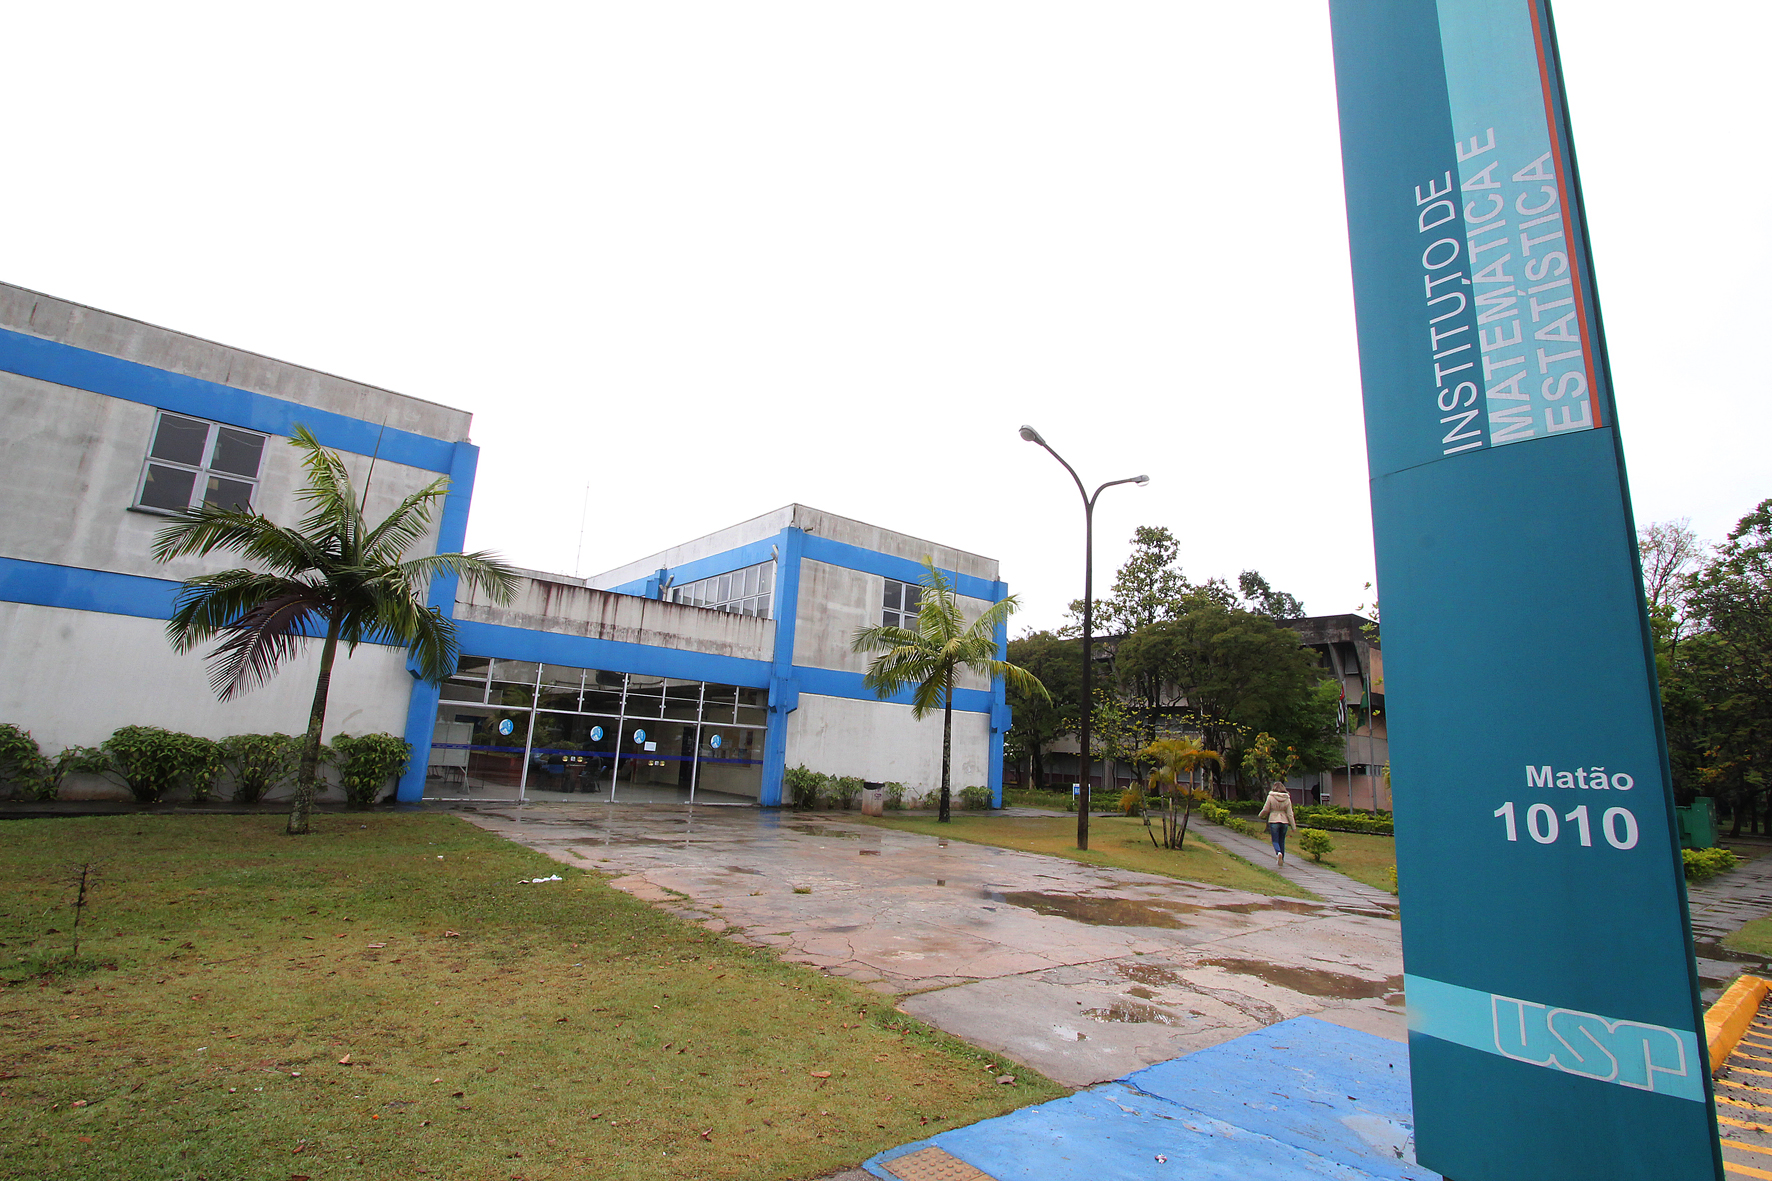
\includegraphics[scale = 0.6]{IME.jpg} % incluí a figura e configura seu tamanho
\caption{\label{fig:IME}Instituto de Matemática e Estatística (IME-USP).} % Legenda
\end{figure}

Para ser aprovado o método de avaliação é feita com média aritmética das \textit{n} Tarefas: EP's e listas. Logo a média final é (1) ou (2):

\begin{equation} % Colocar equação
MF = \frac{1}{n} \sum_{i=1}^{n} T_{n} % média das atividades
\end{equation}

Que pode ser escrita como:

\begin{equation} % Colocar equação
MF = \frac{T_{1} + T_{2} + ... + T_{n}}{n}
\end{equation}

\begin{thebibliography}{refs} % Colocar referências
\bibitem{JupterWeb}
        JupterWeb, Disciplina: MAP2212 - Laboratório de Computação e Simulação.
        \textit{Disponível em:}
        \url{https://uspdigital.usp.br/jupiterweb/obterDisciplina?sgldis=map2212&nomdis=/}
        \textbf {acesso em 06/03/2018.}
        
\bibitem{for LaTeX}
        OETIKER, T. et al, The not so short introduction do \LaTeX (2008).
        \textit{Disponível em:}
        \url{http://ctan.math.washington.edu/tex-archive/info/lshort/english/lshort.pdf/}
        \textbf {acesso em 05/03/2018.}
        
\bibitem{Notas de aula}
        Notas de Aula do professor J. Stern - MAP2212 - Março 2018       
\end{thebibliography}

\end{document}